% Copyright (c) 2014,2016,2018 Casper Ti. Vector
% Public domain.

\chapter{引言}
%\pkuthssffaq % 中文测试文字。

\section{云计算的基本概念}

云计算(Cloud Computing),根据美国国家标准技术研究所(NIST)的定义,指的是一种可以实现对可配置计算资源共享池(如网络、服务器、存储、应用和服务)进行随时随地、便捷、按需网络访问的模型。这些资源可以迅速地配分配和释放,并且这个过程只需要最低限度的资源管理工作以及与服务提供商最少的交互。美国亚马逊公司再2006年3月推出了 Amanzon Web Service(AWS)\parencite{aws},这一事件一般被认为代表着云计算时代的正式开启。经过十几年的发展,凭借着“方便易用、弹性伸缩、按需服务”的技术特征,云计算概念已被广泛接受,云计算产业取得了商业上的巨大成功,云计算平台已成为当今社会的关键信息基础设施,云计算技术为大数据、人工智能的领域的蓬勃发展提供了重要的支撑作用。

\subsection{云计算的传统服务模型}

NIST 将云计算分为了三种服务模型。

这三种服务模型分别是基础设施即服务(Infrastructure as a Service,IaaS)、平台即服务(Platform as a Service,PaaS)以及软件即服务(Software as a Service,SaaS)\parencite{mell2011the}。IaaS为消费者提供用来运行应用的计算资源,包括服务器、存储、网络等。其中虚拟机是云厂商提供的最核心的IaaS产品。与IaaS只提供最基础的底层资源不同,PaaS强调为消费者提供云开发环境,除计算资源以外,PaaS为用户提供中间件开发,运行平台及工具,帮助用户更方便地开、管理、测试和运行应用。SaaS是厂商提供的基于云的软件,用户无需下载安装软件,通过浏览器即可访问服务。

图\ref{rep_products}给出了云计算三种服务模型的代表产品。亚马逊公司的AWS EC2\parencite{awsec2},谷歌公司的Google Compute Engine\parencite{googlecloud}以及阿里云公司的ECS\parencite{aliecs}都是典型的IaaS产品。其主要服务形态是云厂商向消费者售卖虚拟机或者裸金属服务器以及连带的网络、存储等附属产品。PaaS的代表性产品包括AWS Beanstalk、Google App Engine、Microsoft Azure App Servics等。此类产品为用户提供在云中快速部署和管理应用的能力,提供包括应用扩容,负载均衡,应用监控和安全管理等功能。相比于IaaS仅售卖以虚拟机为主的基础设施,PaaS降低了用户开发、管理、运维应用的成本,使得用户可以更加专注于构建应用本身。在云计算已经发展了十几年的当今时代,越来越多的SaaS产品涌现了出来。谷歌公司开发的Google Docs、Google Maps以及微软公司开发的Microsoft Office 365都是典型的SaaS产品。以Google Docs为例,与传统的文件处理办公软降相比,用户无需在本地花费大量存储空间来安装软件,只需要打开浏览器,输入URL,即可使用Google Docs服务处理文件,并且所有的文件都会被及时同步保存到云端。另一个代表性的SaaS产品是Google Maps。Google Maps与Google Docs类似,为个人用户提供在浏览器中直接使用的地图服务。与传统软件相比,SaaS在使用方式上具有方便灵活,跨平台的特性,同时用户存储在云端的数据经过云厂商的冗余备份也具有更高的可靠性。

\begin{figure}
    \centerline{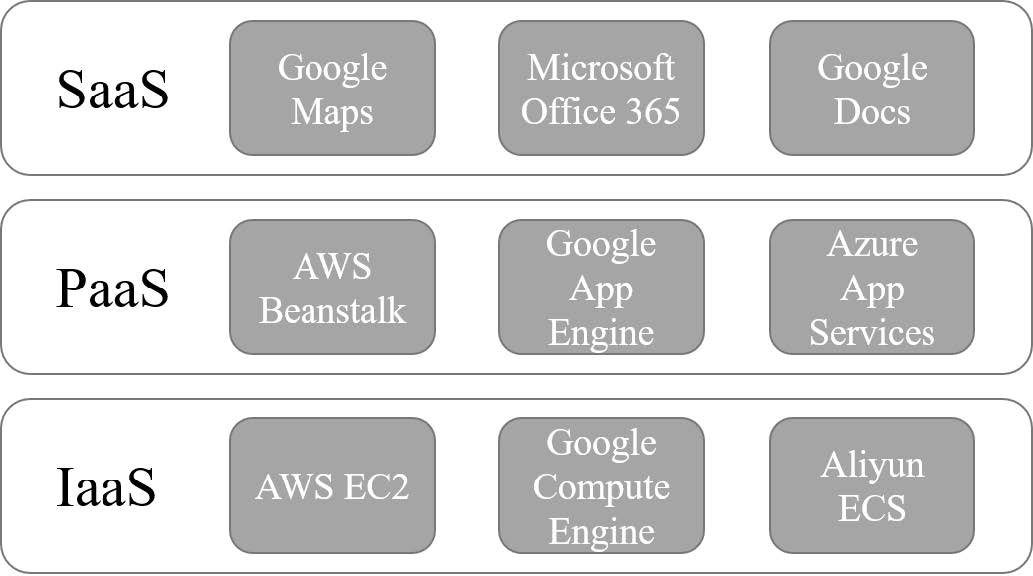
\includegraphics[width=\textwidth]{figures/rep_products.jpg}}
    \caption{云计算服务模型代表产品}
    \label{rep_products}
\end{figure}

\subsection{云计算的新兴服务模型}

云计算发展至今日,其服务模型已经不严格局限于NIST最初总结的这三种基本形态,世界各地各领域的研究者们已经提出了众多不同的X as a Service,包括Blockchain as a Service\parencite{samaniego2016blockchain},Sensing as a Service\parencite{perera2014sensing},Workspace as a Service\parencite{an2017workspace}等。与传统的三种服务形态相比,这些服务不单纯是硬件服务或者软件服务,其结合二者的特点,面向特定的领域方向进行更深度的定制,如区块链、物联网、分布式共识等。服务形态的日益丰富,服务内容的日益复杂体现了云计算更见领域化,精细化的发展趋势。而近几年来最热门的概念莫过于FaaS,即Fucntion as a Service\parencite{baldini2017serverless}。

FaaS是一种新兴的计算模式,亦被称为Serverless Computing。从字面理解,Serverless Computing即为“无服务器计算”之意。然后,其并非意味着真的没有服务器,而已说开发者不用过多考虑服务器的相关问题。在传统的IaaS服务中,开发者需要自己惊醒服务器管理与运维,负责服务的发布,在流量变化时对服务器集群进行扩容或缩容。而在FaaS中,开发者只需要关注业务逻辑,至于服务的发布、管理、弹性伸缩等,则交由云厂商来完成。

FaaS背后的机制一般是以容器技术为基础的。典型地,开发者上传自己的业务代码后,云厂商并不会直接收费。当对该服务的请求到来之时,云厂商将启动一系列容器来运行该服务,从而对用户的请求进行响应。通常而言,开发者指定的服务会与某些时间绑定(hook),在发生该事件时,立即触发开发者定义的服务。我们以AWS的serverless computing服务Lambda\parencite{klems2018aws}中的一个示例程序为例,讲述整个流程。图\ref{aws_resize}所示的是一个为照片调整大小的服务。该服务与AWS S3(AWS的对象存储服务)的上传事件绑定,当云厂商检测到有用户向S3上传图片时,会立即触发开发者定义的图片大小调整函数。整个流程中,开发者需要关注的只有第四步的函数开发工作,至于该函数的横向拓展,全部由云厂商来负责。

\begin{figure}
    \centerline{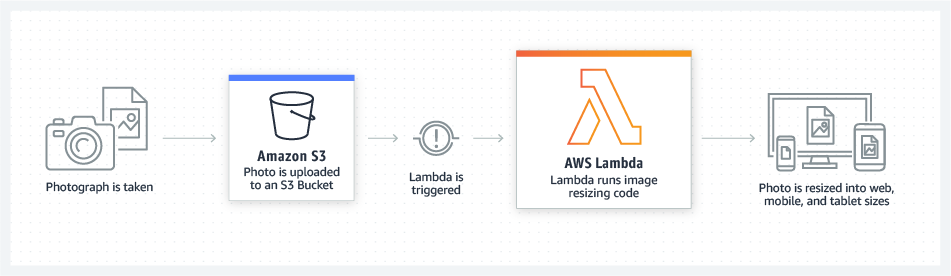
\includegraphics[width=\textwidth]{figures/aws-lambda-resize.png}}
    \caption{AWS Lambda中示例程序:照片大小调整}
    \label{aws_resize}
\end{figure}

主流的云厂商均提供了FaaS服务,例如AWS的Lambda,阿里云的函数计算等,近年来越来越受到开发者的青睐。一方面是因为它的高弹性,易于开发。另一方面则是因为其细粒度的收费模式。通常而言,FaaS的服务是按照请求次数进行收费。当函数闲置时,并不产生额外的费用。

\section{人工智能技术发展简介}\label{sec_ml_history}
人工智能是一个范围很广的概念,广义上的人工智能泛指通过计算机(机器)来实现人的头脑思维,使得机器像人一样区做决策。机器学习是实现人工智能的一种技术途径。一般可以认为人工智能的发展和机器学习技术的进步是同步的,因此,这两个概念大多数场景下会出现在同一个语境中。根据机器学习的发展史,即可勾勒出人工智能领域的发展轨迹,因此本节将简介机器学习技术的发展简史。

虽然机器学习这一名词以及其中某些零碎的方法可以追溯到1958\parencite{samuel1995some}年甚至更早,但真正作为一门独立的学科要从1980年算起,在这一年诞生了第一届机器学习的学术会议和期刊。到目前为止,机器学习的发展经历了3个阶段:1980年代是正式成形期,尚不具备影响力。1990-2010年代是蓬勃发展期,诞生了众多的理论和算法,真正走向了实用。2012年之后是深度学习时期,深度学习技术诞生并急速发展,较好的解决了现阶段AI的一些重点问题,并带来了产业界的快速发展。

\subsection{1980s:登上历史舞台}
十九世纪八十年代,机器学习作为一股独立的力量开始登上历史舞台。此后的十年内,出现了一些重要的方法和理论,典型的代表是:分类与回归树\parencite{breiman1983classification}、反向传播算法\parencite{rumelhart1986learning}和卷积神经网络\parencite{lecun1989backpropagation}。

\textbf{分类与回归树。}分类与回归树由L. Breiman等人在1984年提出,是决策树的一种经典实现,至今它还在很多领域里被使用。决策树是一种基于规则的方法,它由一系列嵌套的规则组成一棵树,完成判断和决策。和之前基于人工规则的方法不同,这里的规则是通过训练得到的,而不是人工总结出来的。

\textbf{反向传播算法。}人工神经网络是对动物神经系统的一种简单模拟,属于仿生方法。从数学的角度看,它是一个多层的复合函数。反向传播算法是神经网络训练时使用的算法,来自于微积分中复合函数求导的链式法则,至今深度学习中各种神经网络的训练使用的还是这种方法。反向传播算法的出现使得多层神经网络真正成为一种可以实现、具有实用价值的算法。在这一时期,神经网络的理论性研究也是热门的问题,神经网络数学上的表达能力的分析和证明大多出现在1980年代末和1990年代初。

从理论上来说,加大神经网络的规模可以解决更复杂的模式识别等问题。但是网络层数的增加会导致梯度消失问题,另外神经网络还面临着局部最优解的问题。训练样本的缺乏,计算能力的限制,都使得神经网络在接下来的20多年里没有太大的进展和出色的表现。

\textbf{卷积神经网络。}早在1989年,Y. LeCun在贝尔实验室就开始使用卷积神经网络识别手写数字\parencite{lecun1989backpropagation},这是当前深度学习中深度卷积神经网络的鼻祖;1998年,LeCun提出了用于字符识别的卷积神经网络LeNet5,并在手写数字识别中取得了较好的结果。卷积神经网络借鉴了动物视觉神经系统的原理,它能够逐层的对输入图像进行抽象和理解。

\subsection{1990-2012:走向成熟和应用}
在这一阶段的20余年里,机器学习的理论和方法得到了完善和充实,代表性的工作包括:支持向量机(SVM)\parencite{cortes1995support}、AdaBoost算法\parencite{freund1995boosting}、循环神经网络(RNN)和长短时记忆网路(LSTM)\parencite{hochreiter1997long}、流形学习\parencite{roweis2000nonlinear}以及随机森林\parencite{breiman2001random}。

\textbf{SVM。}SVM基于最大化分类间隔的原则,通过核函数巧妙的将线性不可分问题转化成线性可分问题,并且具有非常好的泛化性能。和神经网络相比,SVM有完善的数学理论作为支撑,训练时求解的问题是凸优化问题,因此不会出现局部极值问题。

\textbf{AdaBoost。}AdaBoost和随机森林同属集成学习算法,它们通过将多个弱学习器模型整合可以得到精度非常高的强学习器模型,且计算量非常小。AdaBoost算法在机器视觉领域的目标检测问题上取得了成功,典型的代表是人脸检测问题。2001年,使用级联AdaBoost分类器和Haar特征的算法在人脸检测问题上取得了巨大的进步,是有里程碑意义的成果。此后这一框架成为目标检测的主流方法,直到后来被深度学习取代。

\textbf{循环神经网络。}循环神经网络作为标准前馈型神经网络的发展,具有记忆功能,在语音识别、自然语言处理等序列问题的建模上取得了成功,是当前很多深度学习算法的基础。

\textbf{流形学习。}
流形学习作为一种非线性降维技术,直观来看,它假设向量在高维空间中的分布具有一定的几何形状。在2000年出现之后的一段时间内名噪一时,呈现出一片繁荣的景象,但在实际应用方面缺乏成功的建树。

\textbf{随机森林。}
随机森林由Breiman等人在2001年提出,是多棵决策树的集成,在训练时通过对样本进行随机抽样构造出新的数据集训练每一棵决策树。它实现简单,可解释性强,运算量小,在很多实际问题上取得了相当高的精度。时至今日,在很多数据挖掘和分析的比赛中,这类算法还经常成为冠军。

在这一时期机器学习算法真正走向了实际应用。典型的代表是车牌识别,印刷文字、(OCR),手写文字识别,人脸检测技术(数码相机中用于人脸对焦),搜索引擎中的自然语言处理技术和网页排序,广告点击率预估(CTR),推荐系统,垃圾邮件过滤等。

\subsection{2012之后:深度学习时代来临}
在与SVM的竞争中,神经网络长时间内处于下风,直到2012年\parencite{krizhevsky2017imagenet}局面才被改变。SVM、AdaBoost等所谓的浅层模型并不能很好的解决图像识别,语音识别等复杂的问题,在这些问题上存在严重的过拟合。为此产业界需要更强大的算法,历史又一次选择了神经网络。

由于算法的改进以及大量训练样本的支持,加上计算能力的进步,训练深层、复杂的神经网络成为可能,它们在图像、语音识别等有挑战性的问题上显示出明显的优势。

深度学习的再度兴起可以追溯到2006年,G. Hinton等人\parencite{hinton2006reducing}提出了一种训练深层神经网络的方法,用受限玻尔兹曼机训练多层神经网络的每一层,得到初始权重,然后继续训练整个神经网络。2012年Hinton小组发明的深度卷积神经网络AlexNet\parencite{krizhevsky2017imagenet}首先在图像分类问题上取代成功,随后被用于机器视觉的各种问题上,包括通用目标检测,人脸检测,行人检测,人脸识别,图像分割,图像边缘检测等。在这些问题上,卷积神经网络取得了当前最好的性能。在另一类称为时间序列分析的问题上,循环神经网络取得了成功。典型的代表是语音识别,自然语言处理,使用深度循环神经网络之后,语音识别的准确率显著提升,直至达到实际应用的要求。

与此同时,在策略、控制类问题上,深度强化学习技术取得了成功,典型的代表是AlphaGo\parencite{silver2016mastering}。在各种游戏、自动驾驶等问题上,深度强化学习显示出了接近人类甚至比人类更强大的能力。另外,以生成对抗网络(GAN)\parencite{goodfellow2014generative}为代表的深度生成框架在数据生成方面取得了惊人的效果,可以创造出逼真的图像,流畅的文章,动听的音乐,为解决数据生成这种“创作”类问题开辟了一条新思路。这一时期AI的产业化明显加速,人工智能已经成为当前计算机科学领域最炙手可热的方向。随着机器学习任务的规模越来越大,其对算力的要求也越来越高,大量机器学习任务开始向有着近乎无限资源的公有云迁移。

\section{云计算和人工智能交叉领域的常见研究问题}
云计算和人工智能是两个息息相关的热门领域。一方面,以深度学习为典型代表的人工智能技术在当今社会被应用的越来越广泛,研发、调试、发布新的模型的需求日益增长。与这种发展趋势对应,多数主流的云厂商都提供了机器学习模型训练-测试-部署的pipeline。学术界也不断探索“云上机器学习”这一话题,在各种不同的业务场景下,利用不同的云服务更便捷、更经济高效地在公有云上开展ML模型的训练和部署。同时得益于近年硬件技术的发展,多种异构硬件在云环境中得到应用,为提升机器学习任务的性能和增强机器学习任务的安全型提供了新的可能。另一方面,机器学习技术也越来越多被用于解决云计算中常见的问题。例如使用机器学习算法解决置优化问题和利用强化学习解云环境中的资源调度问题。下文对这几个常见问题做简单概述,具体研究将在后续几章展开。

\subsection{基于公有云服务的机器学习平台}
\subsubsection{产业界的一站式系统}

主流的云厂商都提供了面向机器学习的平台系统,例如AWS和Sagamaker\parencite{joshi2020amazon,liberty2020elastic,perrone2020amazon},Azure的Azure ML Studio\parencite{etaati2019azure},腾讯的Angel\parencite{jiang2018angel}等。这些基于云的平台提供了一站式调试、训练和部署ML模型的能力。一般而言此类平台被视为SaaS类的服务,因为其是基于云资源构建的上层软件栈,使得用户能够直接使用web的方式使用。例如Sagemaker就支持用户直接在浏览器中用jupyter notebook编写和调试模型代码。

\subsubsection{基于传统云服务的第三方系统}

一般而言,产业界的平台系统面向的是用户最普遍的需求。因此,对于有特殊需求的用户,通常会有与产业界的解决方案并行的工作。例如,为了以尽可能低的成本在云上完成模型的训练,相关工作\parencite{harlap2017proteus,li2020spottune}尝试利用云上的动态资源(价格低但是稳定性/可用性低)进行模型的训练,并辅以一定的策略增强其可靠性。再比如,机器学习模型的在线服务会有低延迟、高吞吐率的要求。为了实现上述需求,相关工作\parencite{zhang2019mark}利用云上的多种资源,根据负载的动态变化,敏捷地在不同资源之间切换,充分利用不同类型资源的优点,规避掉其缺点,实现高效、经济的模型在线服务。一般而言,学术界的此类研究构建于云厂商服务的上层,是一种Cloud-of-Clouds的模式。

\subsubsection{基于新兴云服务的第三方系统}

以FaaS为代表的新型云计算模式,以其高弹性、灵活的计费方式等特点吸引了众多研究者的注意。一般而言,用来训练机器学习模型的集群大小是固定的,很难动态地进行伸缩。同时,开发者还需要自行对该集群进行维护和管理,从而徒增一些不必要地时间和人力开销。因此,学术界开始探讨如何使得机器学习工作流享用到FaaS的诸多优点\parencite{wang2019distributed},从而使得其计算资源在模型训练时能按需伸缩,结束训练后自动将模型存储在持久化存储中,计算资源随即释放。

除了模型训练,也有部分研究者尝试利用FaaS,以serverless的模式部署模型。虽然这一想法非常自然,但是还有诸多问题需要解决。例如,现有的serverless服务,如AWS Lambda,其单个instance所能使用的内存有限,也无法使用GPU等加速芯片,同时其冷启动时间也较长(相比于服务对latency的要求)。如何优化FaaS的系统架构,使其更适合模型的部署,也是一个值得研究的问题。

\subsection{异构硬件对人工智能的影响}
根据\ref{sec_ml_history}中的描述,人工神经网络早在上世纪80年代就被提出。然而直到本世纪10年代左右,神经网络才再次进入学术界和产业界的视野,并得到了飞速发展。除了理论的进步,更重要的原因是算力的大幅进步。以GPU,FPGA为代表的并行化加速硬件,极大地加快了深度学习模型的训练速度,使得学术界对于新模型架构的探索周期大幅缩短。在这种背景下,除了深度学习算法理论的迭代加快,也催生了一批针对机器学习系统的研究工作。这些工作关注如何使异构的硬件更好地支持机器学习模型的训练。

除了训练速度,安全也是人工智能领域的一个重要问题。当今时代数据已经成为重要的资产,开发者在将机器学习任务部署到云端的同时,也会对数据的安全性有所担忧。虽然诸如同态加密之类的软件层面的解决方案可以提升ML任务的安全性,但是由于性能的制约始终未能得到大规模应用。以Intel SGX\parencite{costan2016intel}为代表的安全计算环境技术,给人工智能安全带来了新的解决方案。


\subsection{利用机器学习算法解决云计算中的资源配置与调度问题}
\subsubsection{利用机器学习算法解决配置优化问题}

公有云厂商所提供的计算资源类型和计费模式越来越复杂。据不完全统计,截至目前,AWS EC2提供了超过400种配置的虚拟机,阿里云提供了超过500种虚拟机。除了虚拟机配置不同之外,其收费模型也存在多种。例如,除了传统的包年包月、按量付费等,还有抢占式实例(在AWS中成为Spot Instance)\parencite{awsspot}等计费方式。在此场景中,用户所面临的一个重要问题在于如何为自己的应用程序/负载选择合适配置和收费方式的资源。

部分研究者利用机器学习算法来解决此类问题。有的将其看作一个推荐问题\parencite{klimovic2018selecta},用协同过滤等推荐系统中常用的算法为不同的应用程序匹配合适的配置。有的将其建模为回归问题\parencite{yadwadkar2017selecting,venkataraman2016ernest,moradi2019performance,zheng2019online},将应用程序的信息、资源的配置信息等作为输入,预测在某种配置下某个应用程序的性能或者花费,从而得到最佳的配置。还有的将其视作在线优化问题\parencite{alipourfard2017cherrypick,casimiro2019lynceus},利用贝叶斯优化等方法,通过有限次的尝试逐渐逼近最优解。

\subsubsection{利用机器学习算法解决资源调度问题}

资源调度是操作系统、分布式系统和云计算领域中的经典问题,其本质在于为系统中的每个任务分配合适的资源,从而使得系统达到某种状态,如资源利用率最高、闲置资源最少或者吞吐率最高等。近年来深度学习的流行,尤其是强化学习的兴起,使得部分研究者开始思考利用机器学习算法解决资源调度问题\parencite{delimitrou2014quasar,mao2019learning,chung2018stratus}。一般而言,此类算法旨在从过去的任务执行记录中“学习”相关的规律,以指导为未来系统的调度动作。
% vim:ts=4:sw=4
